\documentclass[]{informeutn}

% Bibliografía
\usepackage[backend=bibtex, style=alphabetic, sorting=ynt]{biblatex}
\addbibresource{fuentes.bib}

% Paquetes adicionales
\usepackage{subcaption}

% Unidades personalizadas adicionales a las de la clase
\newcommand{\lux}{\,\mathrm{lx}}
\newcommand{\lumen}{\,\mathrm{lm}}
\newcommand{\cd}{\,\mathrm{cd}}
\newcommand{\m}{\,\mathrm{m}}
\newcommand{\lx}{\,\mathrm{lx}}
\newcommand{\lm}{\,\mathrm{lm}}
\newcommand{\nm}{\,\mathrm{nm}}
\newcommand{\cm}{\,\mathrm{cm}}

% Configuración de datos del informe
\materia{Seguridad, Higiene y Medio Ambiente}
\titulo{Trabajo Práctico Nº 2}
\subtitulo{Medición y Evaluación de Iluminación en el Ambiente Laboral}
\comision{4R2} % Puede modificarse según la comisión real
\autores{Franco Palombo - 401910}
\fecha{3 de Julio de 2026}

\begin{document}

\maketitle

\tableofcontents
\setcounter{page}{1}
\thispagestyle{plain}
\usetikzlibrary{patterns}.

% Capítulos del informe
\chapter{Introducción}
\label{sec.tp2:introduccion}

La iluminación en los ámbitos laborales constituye uno de los factores ambientales de mayor relevancia para la
seguridad, salud y productividad de los trabajadores. Un sistema de iluminación inadecuado puede generar fatiga visual,
cefaleas, errores operativos e incluso incrementar significativamente la tasa de siniestralidad. Por el contrario, un
nivel y calidad óptimos de iluminación favorecen el desempeño cognitivo y motor, disminuyendo el cansancio y previniendo
accidentes.

En la República Argentina, el marco normativo establece criterios técnicos estrictos para asegurar condiciones dignas
de iluminación. El Decreto N° 351/79, reglamentario de la Ley de Higiene y Seguridad en el Trabajo N° 19.587,
determina las intensidades mínimas de iluminación requeridas según el tipo de edificio, local y tarea visual en su
Anexo IV. Asimismo, la Resolución SRT N° 84/2012 estipula un protocolo de carácter obligatorio para registrar y evaluar
las mediciones de iluminación en los puestos de trabajo.

\section{Objetivos}
\label{sec.tp2:objetivos}

Los objetivos principales de este trabajo práctico son:
\begin{itemize}
    \item Relevar el sistema de iluminación actual en un ambiente real seleccionado.
    \item Calcular las dimensiones del local y determinar la grilla de medición conforme a las exigencias normativas de la Resolución SRT N° 84/2012.
    \item Medir los niveles de iluminancia utilizando un instrumento de medición adecuado (luxómetro o aplicación calibrada).
    \item Determinar la iluminancia media ($E_{media}$) y verificar la relación de uniformidad del local.
    \item Comparar los resultados con las exigencias del Decreto N° 351/79 para evaluar la conformidad.
    \item Elaborar conclusiones técnicas y, si corresponde, proponer mejoras en la instalación.
\end{itemize}

\chapter{Fundamentos Teóricos Acotados}
\label{sec.tp2:teoria}

En esta sección se presentan resumidas las magnitudes y fórmulas luminotécnicas fundamentales aplicadas en el desarrollo
y evaluación del informe.

\section{Magnitudes y Fórmulas Fundamentales}
\label{sec.tp2:magnitudes}

Las magnitudes y relaciones matemáticas utilizadas para caracterizar el ambiente de trabajo son:

\begin{itemize}
    \item \textbf{Flujo Luminoso ($\Phi$):} Potencia luminosa visible emitida por una fuente. Su unidad es el lumen ($\lm$).
    
    \item \textbf{Intensidad Luminosa ($I$):} Flujo emitido por unidad de ángulo sólido ($\omega$) en una dirección dada. Unidad: candela ($\cd$).
    \begin{equation}
        I = \frac{d\Phi}{d\omega}
        \label{eq.tp2:intensidad}
    \end{equation}
    
    \item \textbf{Iluminancia ($E$):} Densidad de flujo luminoso que incide sobre una superficie ($S$). Unidad: lux ($\lx = \lm/\m^2$).
    \begin{equation}
        E = \frac{\Phi}{S}
        \label{eq.tp2:iluminancia}
    \end{equation}
    
    \item \textbf{Eficacia Lumínica ($\eta$):} Relación entre el flujo emitido y la potencia eléctrica ($P$) consumida. Unidad: $\lm/\W$.
    \begin{equation}
        \eta = \frac{\Phi}{P}
        \label{eq.tp2:eficacia}
    \end{equation}
\end{itemize}

\section{Leyes de la Luminotecnia}
\label{sec.tp2:leyes}

\begin{itemize}
    \item \textbf{Ley de la Inversa de los Cuadrados:} Determina la iluminancia producida por una fuente puntual sobre un plano perpendicular a una distancia ($d$):
    \begin{equation}
        E = \frac{I}{d^2}
        \label{eq.tp2:inversa_cuadrados}
    \end{equation}
    
    \item \textbf{Ley del Coseno (Lambert):} Calcula la iluminancia sobre un plano horizontal ($E_H$) cuando el haz incide con un ángulo $\theta$ respecto a la normal del plano, a una altura de montaje ($h$):
    \begin{equation}
        E_H = \frac{I_\theta \cdot \cos^3\theta}{h^2}
        \label{eq.tp2:ley_coseno}
    \end{equation}
\end{itemize}

\section{Marco Legal Aplicable}
\label{sec.tp2:marco_legal}

\begin{itemize}
    \item \textbf{Decreto N° 351/79 (Anexo IV):} Exige intensidades medias de iluminación mínimas según la tarea visual, además de fijar el criterio de uniformidad para la iluminancia mínima ($E_{min}$) e iluminancia media ($E_{media}$):
    \begin{equation}
        E_{min} \ge \frac{E_{media}}{2}
        \label{eq.tp2:uniformidad_lim}
    \end{equation}
    
    \item \textbf{Resolución SRT N° 84/2012:} Define el protocolo obligatorio y la metodología de grilla para evaluar el nivel general de iluminación en los ambientes de trabajo.
\end{itemize}

\chapter{Metodología de Medición}
\label{sec.tp2:metodologia}

Para determinar el nivel de iluminación general de un local interior de forma representativa, la Resolución SRT N°
84/2012 adopta la metodología de la grilla (o método de la cuadrícula). Este método consiste en dividir la superficie
del suelo en zonas cuadradas o rectangulares de igual área y realizar mediciones en el centro de cada una de ellas a la
altura del plano de trabajo (usualmente a $0{,}8\m$ sobre el nivel del piso).

\section{Determinación del Número de Puntos de Muestreo}
\label{sec.tp2:determinacion_puntos}

El número mínimo de puntos de medición necesarios para una adecuada caracterización depende de la relación dimensional del
ambiente, la cual está expresada a través del Índice del Local ($k$). Este índice se calcula mediante la relación:
\begin{equation}
    k = \frac{a \cdot b}{h_m \cdot (a + b)}
    \label{eq.tp2:indice_k}
\end{equation}
Donde:
\begin{itemize}
    \item $a$: ancho del local (medido en metros, $\m$).
    \item $b$: largo del local (medido en metros, $\m$).
    \item $h_m$: altura de montaje de las luminarias con respecto al plano de trabajo (medida en metros, $\m$). Se calcula como la altura total de las luminarias ($H$) menos la altura del plano de trabajo ($h_p = 0{,}8\m$).
\end{itemize}

Posteriormente, el valor del índice $k$ se redondea al entero superior inmediato ($k_{red}$), considerando que:
\begin{itemize}
    \item Si $k \le 1$, entonces $k_{red} = 1$.
    \item Si $1 < k \le 2$, entonces $k_{red} = 2$.
    \item Si $2 < k \le 3$, entonces $k_{red} = 3$.
    \item Si $k > 3$, entonces $k_{red} = 4$.
\end{itemize}

Con el valor de $k_{red}$ determinado, el número mínimo de puntos de medición ($N$) a relevar se calcula con la
siguiente fórmula:
\begin{equation}
    N = (k_{red} + 2)^2
    \label{eq.tp2:num_puntos}
\end{equation}

El resultado determina una grilla regular de medición, cuyas configuraciones típicas son:
\begin{itemize}
    \item Para $k_{red} = 1$: grilla de $3 \times 3$ ($N = 9$ puntos).
    \item Para $k_{red} = 2$: grilla de $4 \times 4$ ($N = 16$ puntos).
    \item Para $k_{red} = 3$: grilla de $5 \times 5$ ($N = 25$ puntos).
    \item Para $k_{red} = 4$: grilla de $6 \times 6$ ($N = 36$ puntos).
\end{itemize}

Cuando el local analizado posee una planta de geometría irregular, este se subdivide en sectores rectangulares o
cuadrados individuales y se aplica el método de la grilla de forma independiente para cada sector.

\section{Procedimiento para el Relevamiento}
\label{sec.tp2:procedimiento}

Una vez calculada la grilla de medición y la cantidad de puntos, se procede de la siguiente manera en el local:
\begin{enumerate}
    \item Se proyecta la cuadrícula sobre el piso del ambiente y se localizan los centros geométricos de cada área elemental.
    \item Las mediciones se ejecutan a la altura del plano de trabajo ($0{,}8\m$ sobre el suelo para tareas generales).
    \item Para evitar interferencias en el sensor del instrumento (luxómetro o sensor móvil), el operador debe evitar proyectar sombras propias sobre el elemento sensor y vestir ropa de color neutro u oscuro en la medida de lo posible.
    \item Se registra la iluminancia en cada punto en un horario de actividad normal del local (contemplando la combinación de luz artificial y luz natural si aplica, o exclusivamente artificial de noche).
\end{enumerate}

\section{Cálculos de Evaluación}
\label{sec.tp2:calculos_evaluacion}

A partir de los niveles de iluminancia obtenidos ($E_1, E_2, \dots, E_N$), se realizan los siguientes cálculos:

\subsection{Iluminancia Media \texorpdfstring{($E_{media}$)}{(E\_media)}}
Es el promedio aritmético simple de los valores registrados en los $N$ puntos de la cuadrícula:
\begin{equation}
    E_{media} = \frac{1}{N} \sum_{i=1}^{N} E_i
    \label{eq.tp2:iluminancia_media}
\end{equation}

\subsection{Uniformidad de la Iluminación}
Se identifica el valor mínimo absoluto registrado ($E_{min}$). Para verificar el cumplimiento del criterio de uniformidad exigido por el Decreto N° 351/79, se evalúa si:
\begin{equation}
    E_{min} \ge \frac{E_{media}}{2}
    \label{eq.tp2:verificacion_uniformidad}
\end{equation}
Si la desigualdad se cumple, la distribución de luz en el local se considera uniforme.

\chapter{Desarrollo del Relevamiento}
\label{sec.tp2:desarrollo}

En esta sección se detallan las características constructivas de la habitación relevada (compuesta por dos sectores: la
oficina y el depósito), se definen las especificaciones del sistema de iluminación (general y localizado) y se
desarrollan los cálculos normativos para el dimensionamiento de las grillas de medición.

\section{Descripción del Local y Geometría}
\label{sec.tp2:descripcion_local}

El local relevado se encuentra dividido en dos espacios diferenciados de geometría regular: la oficina (área grande) y
el depósito (área chica). El techo de toda la habitación se encuentra a una altura uniforme de $2{,}50\m$ desde el
piso. La reflectancia de las paredes es media-alta (blanco mate) y el suelo es de cerámicos claros.

Las dimensiones geométricas de ambos sectores son:
\begin{itemize}
    \item \textbf{Oficina (Sector Principal):}
    \begin{itemize}
        \item Ancho ($a_{of}$): $3{,}28\m$
        \item Largo ($b_{of}$): $3{,}52\m$
    \end{itemize}
    \item \textbf{Depósito (Sector Secundario):}
    \begin{itemize}
        \item Ancho ($a_{dep}$): $1{,}15\m$
        \item Largo ($b_{dep}$): $1{,}92\m$
    \end{itemize}
    \item \textbf{Alturas de Referencia:}
    \begin{itemize}
        \item Altura total del techo ($H$): $2{,}50\m$
        \item Altura del plano de trabajo ($h_p$): $0{,}80\m$ (altura de los escritorios)
        \item Altura de montaje de luminarias generales ($H_{lum}$): $2{,}50\m$ (montadas directamente al techo)
    \end{itemize}
\end{itemize}

En la oficina se encuentran dos escritorios: un escritorio de trabajo principal de dimensiones extensas ($1{,}88\m \times 0{,}50\m$) ubicado contra la pared izquierda, y un escritorio secundario pequeño de ($1{,}20\m \times 0{,}76\m$) ubicado en la esquina superior derecha.

\section{Especificaciones del Sistema de Iluminación}
\label{sec.tp2:especificaciones_luces}

Todas las fuentes de luz instaladas en los dos sectores corresponden a tecnología LED de temperatura de color blanca fría ($\ge 6000\Kelvin$). El sistema se divide en iluminación general e iluminación localizada:

\subsection{Iluminación General (Techo)}
\begin{itemize}
    \item \textbf{Luminaria General Oficina (P1):} Un ($1$) plafón LED de adosar de $18\W$, luz fría, ubicado en el centro geométrico del cielorraso de la oficina.
    \item \textbf{Luminaria General Depósito (P2):} Un ($1$) plafón LED de adosar de $18\W$, luz fría, ubicado en el centro geométrico del cielorraso del depósito.
\end{itemize}

\subsection{Iluminación Localizada (Escritorios)}
\begin{itemize}
    \item \textbf{Escritorio Largo (Pared Izquierda):} Equipado con una tira LED 5050 monocolor fría de punta a punta ($1{,}88\m$). Presenta una densidad de 3 leds cada $5\cm$ ($60\text{ leds}/\m$, totalizando $113$ leds). Está montada en un perfil de aluminio a $62\cm$ sobre el plano de trabajo (altura respecto al piso $h = 1{,}42\m$). Consumo estimado de $14{,}4\W/\m$ (potencia de la tira $\approx 27\W$) y un flujo total de $\approx 1800\lumen$.
    \item \textbf{Escritorio Chico (Esquina Superior Derecha):} Equipado con una luminaria de mesa regulable LED, luz fría, con un flujo luminoso máximo de $700\lumen$ y una potencia aproximada de $18\W$, montada de forma centrada a una altura de $65\cm$ sobre el plano de trabajo (altura respecto al piso $h = 1{,}45\m$).
\end{itemize}

\section{Cálculo del Índice del Local y Puntos de Medición}
\label{sec.tp2:calculo_grilla}

La altura de montaje de las luminarias generales respecto al plano de trabajo es:
\begin{equation}
    h_m = H_{lum} - h_p = 2{,}50\m - 0{,}80\m = 1{,}70\m
\end{equation}

Se realizan los cálculos del Índice de Local ($k$) y de la cantidad de puntos de medición mínimos ($N$) de forma independiente para cada área:

\subsection{Área de Oficina (Grande)}
\begin{equation}
    k_{oficina} = \frac{3{,}28\m \cdot 3{,}52\m}{1{,}70\m \cdot (3{,}28\m + 3{,}52\m)} = \frac{11{,}5456}{11{,}56} \approx 1{,}00
\end{equation}
Dado que $k \le 1$, el índice redondeado es $k_{red} = 1$. La cantidad mínima de puntos de medición se calcula como:
\begin{equation}
    N_{oficina} = (1 + 2)^2 = 9\text{ puntos (grilla de } 3 \times 3\text{)}
\end{equation}
Las celdas resultantes de la división tienen dimensiones de $1{,}173\m$ de largo por $1{,}093\m$ de ancho.

\subsection{Área de Depósito (Chico)}
\begin{equation}
    k_{deposito} = \frac{1{,}15\m \cdot 1{,}92\m}{1{,}70\m \cdot (1{,}15\m + 1{,}92\m)} = \frac{2{,}208}{5{,}219} \approx 0{,}42
\end{equation}
Dado que $k \le 1$, el índice redondeado es $k_{red} = 1$. El número mínimo de puntos de medición general es:
\begin{equation}
    N_{deposito} = (1 + 2)^2 = 9\text{ puntos (grilla de } 3 \times 3\text{)}
\end{equation}
Las celdas resultantes de la división tienen dimensiones de $0{,}64\m$ de largo por $0{,}383\m$ de ancho.

\subsection{Puntos de Iluminación Localizada}
Para verificar el aporte lumínico localizado, se realizaron mediciones directas sobre los escritorios:
\begin{itemize}
    \item En el escritorio largo se determinan 3 puntos equidistantes distribuidos a lo largo del mismo ($E_{L1}, E_{L2}, E_{L3}$).
    \item En el escritorio chico se determina 1 punto centrado en el área de trabajo ($E_{C1}$).
\end{itemize}

\section{Croquis e Implantación del Local}
\label{sec.tp2:croquis}

El croquis detallado de planta de la habitación, con la delimitación de ambos sectores (oficina y depósito), la ubicación de los escritorios, las luminarias generales y localizadas, y la grilla de medición resultante, se representa en la Figura~\ref{fig.tp2:croquis_habitacion}.

\begin{figure}[!ht]
    \centering
    \begin{tikzpicture}[scale=2.0, >=latex]
    % === ESTILOS ===
    \tikzstyle{wall} = [black, line width=2.0pt]
    \tikzstyle{desk} = [pattern=north west lines, pattern color=gray!30, draw=gray, line width=0.8pt]
    \tikzstyle{window} = [blue!80!black, line width=2.5pt, double, double distance=1.5pt]
    \tikzstyle{cota} = [gray!80!black, thin, <->]
    \tikzstyle{cotaline} = [gray!40, thin]
    \tikzstyle{gridline} = [blue!15, dashed, ultra thin]

    % === INDICACIÓN DEL SUR (A LA IZQUIERDA DEL CROQUIS) ===
    \draw[thick, ->] (-0.5, 1.64) -- (-0.9, 1.64) node[left, font=\bfseries\small] {SUR};

    % === DIBUJO DE PISO Y PAREDES ===
    \fill[gray!2] (0,0) -- (0,3.28) -- (3.52,3.28) -- (3.52,0) -- cycle;
    \fill[gray!4] (0.54,3.28) -- (0.54,5.32) -- (1.69,5.32) -- (1.69,3.28) -- cycle;

    % Paredes externas
    \draw[wall] (0,0) -- (0,1.88) -- (0.34, 1.88) -- (0.34, 2.25) -- (0, 2.25) -- (0, 3.28) 
                -- (0.54, 3.28) -- (0.54, 5.32) -- (1.69, 5.32) -- (1.69, 3.28) 
                -- (3.52, 3.28) -- (3.52, 0) -- (0,0);

    % Ventanas
    \draw[window] (.65, 0) -- ++(.62, 0);
    \draw[window] (3.52, .7) -- ++(0, 1.88);

    % === MUEBLES (ESCRITORIOS) ===
    \draw[desk] (0, 0) rectangle (0.5, 1.88);
    \draw[desk] (3.52, 3.28) rectangle (2.76, 2.08);

    % === GRILLES DE MEDICIÓN GENERAL (LÍNEAS DE TRAZOS) ===
    \foreach \x in {1.173, 2.346} {
        \draw[gridline] (\x, 0) -- (\x, 3.28);
    }
    \foreach \y in {1.093, 2.186} {
        \draw[gridline] (0, \y) -- (3.52, \y);
    }

    \foreach \x in {0.923, 1.306} {
        \draw[gridline] (\x, 3.40) -- (\x, 5.32);
    }
    \foreach \y in {4.04, 4.68} {
        \draw[gridline] (0.54, \y) -- (1.69, \y);
    }

    % Puntos de Iluminación Localizada - Cruces Rojas
    \foreach \py/\pnum in {0.31/1, 0.94/2, 1.57/3} {
        \draw[red!85!black, thick] (0.25-0.05, \py) -- (0.25+0.05, \py);
        \draw[red!85!black, thick] (0.25, \py-0.05) -- (0.25, \py+0.05);
        \node[right, scale=0.5, red!70!black] at (0.27, \py) {$E_{L\pnum}$};
    }
    \draw[red!85!black, thick] (3.14-0.05, 2.68) -- (3.14+0.05, 2.68);
    \draw[red!85!black, thick] (3.14, 2.68-0.05) -- (3.14, 2.68+0.05);
    \node[above left, scale=0.5, red!70!black] at (3.12, 2.68) {$E_{C1}$};

    % === LUMINARIAS (SIN TEXTOS DE ACLARACIÓN ADENTRO) ===
    % 1. Plafón General Oficina (Centrado en Oficina: 1.76, 1.64)
    \draw[fill=cyan!10, draw=cyan!80!black, double, thick] (1.76, 1.64) circle (0.10);
    \draw[cyan!80!black, thin] (1.76-0.10, 1.64) -- (1.76+0.10, 1.64);
    \draw[cyan!80!black, thin] (1.76, 1.64-0.10) -- (1.76, 1.64+0.10);

    % 2. Plafón General Depósito (Centrado en Depósito: 1.115, 4.36)
    \draw[fill=cyan!10, draw=cyan!80!black, double, thick] (1.115, 4.36) circle (0.10);
    \draw[cyan!80!black, thin] (1.115-0.10, 4.36) -- (1.115+0.10, 4.36);
    \draw[cyan!80!black, thin] (1.115, 4.36-0.10) -- (1.115, 4.36+0.10);

    % 3. Tira LED Escritorio Largo (x=0.25, de y=0.1 a y=1.78)
    \draw[yellow!80!orange, line width=2.2pt, cap=round] (0.25, 0.1) -- (0.25, 1.78);

    % 4. Luminaria Regulable Escritorio Chico (Centrado en Escritorio Chico: 3.14, 2.68)
    \draw[fill=yellow!20, draw=yellow!80!orange, thick] (3.14, 2.68) circle (0.07);
    \draw[yellow!80!orange, fill=yellow!80!orange] (3.14, 2.68) circle (0.02);


    % === PUNTOS DE MEDICIÓN ===
    % Puntos Oficina (E1 a E9) - Círculos Naranjas
    \def\ox{3.52/3}
    \def\oy{3.28/3}
    \foreach \ix in {1,2,3} {
        \foreach \iy in {1,2,3} {
            \pgfmathsetmacro{\px}{(\ix - 0.5) * \ox}
            \pgfmathsetmacro{\py}{(\iy - 0.5) * \oy}
            \pgfmathsetmacro{\pnum}{int((\iy - 1) * 3 + \ix)}
            \fill[orange!85!black] (\px, \py) circle (0.04);
            \node[below, scale=0.8, orange!65!black] at (\px, \py) {$E_{\pnum}$};
        }
    }

    % Puntos Depósito (E10 a E18) - Círculos Naranjas
    \def\dx{1.15/3}
    \def\dy{1.92/3}
    \foreach \ix in {1,2,3} {
        \foreach \iy in {1,2,3} {
            \pgfmathsetmacro{\px}{0.54 + (\ix - 0.5) * \dx}
            \pgfmathsetmacro{\py}{3.40 + (\iy - 0.5) * \dy}
            \pgfmathsetmacro{\pnum}{int(9 + (\iy - 1) * 3 + \ix)}
            \fill[orange!85!black] (\px, \py) circle (0.04);
            \node[below, scale=0.8, orange!65!black] at (\px, \py) {$E_{\pnum}$};
        }
    }

    % === TEXTOS / ROTULACIÓN DE AREAS ===
    \node[scale=0.8, font=\bfseries, text=gray!70] at (1.76, 1) {OFICINA};
    \node[scale=0.8, font=\bfseries, text=gray!70] at (1.115, 4.65) {DEPÓSITO};

    % === COTAS ===
    \draw[cotaline] (0,0) -- (0,-0.25);
    \draw[cotaline] (3.52,0) -- (3.52,-0.25);
    \draw[cota] (0,-0.20) -- (3.52,-0.20) node[midway, fill=white, scale=0.7] {$3{,}52\m$};

    \draw[cotaline] (3.52,0) -- (3.77,0);
    \draw[cotaline] (3.52,3.28) -- (3.77,3.28);
    \draw[cota] (3.72,0) -- (3.72,3.28) node[midway, rotate=-90, fill=white, scale=0.7] {$3{,}28\m$};

    \draw[cotaline] (0.54,5.32) -- (0.54,5.57);
    \draw[cotaline] (1.69,5.32) -- (1.69,5.57);
    \draw[cota] (0.54,5.52) -- (1.69,5.52) node[midway, fill=white, scale=0.7] {$1{,}15\m$};

    \draw[cotaline] (0.54,3.28) -- (0.29,3.28);
    \draw[cotaline] (0.54,5.32) -- (0.29,5.32);
    \draw[cota] (0.34,3.28) -- (0.34,5.32) node[midway, rotate=90, fill=white, scale=0.7] {$1{,}92\m$};

    \draw[cotaline] (0,1.88) -- (0.45,1.88);
    \draw[cotaline] (0,2.25) -- (0.45,2.25);
    \draw[cota] (0.40,1.88) -- (0.40,2.25) node[midway, right, scale=0.55] {$0{,}37\m$};
    
    \draw[cotaline] (0,1.88) -- (0,2.35);
    \draw[cotaline] (0.34,1.88) -- (0.34,2.35);
    \draw[cota] (0,2.30) -- (0.34,2.30) node[midway, above, scale=0.55] {$0{,}34\m$};

    % === LISTA DE REFERENCIAS AL COSTADO (SIN LÍNEA PUNTEADA NI DE PARED) ===
    \node[anchor=west] at (4.0, 4.8) {\textbf{Referencias:}};
    
    % Plafón LED General
    \draw[fill=cyan!10, draw=cyan!80!black, double, thick] (4.2, 4.4) circle (0.08);
    \draw[cyan!80!black, thin] (4.2-0.08, 4.4) -- (4.2+0.08, 4.4);
    \draw[cyan!80!black, thin] (4.2, 4.4-0.08) -- (4.2, 4.4+0.08);
    \node[anchor=west, scale=0.7] at (4.5, 4.4) {Plafón LED General (18W)};
    
    % Tira LED Localizada
    \draw[yellow!80!orange, line width=2.5pt, cap=round] (4.1, 3.9) -- (4.3, 3.9);
    \node[anchor=west, scale=0.7] at (4.5, 3.9) {Tira LED Localizada (5050)};
    
    % Luminaria Focalizada
    \draw[fill=yellow!20, draw=yellow!80!orange, thick] (4.2, 3.4) circle (0.06);
    \draw[yellow!80!orange, fill=yellow!80!orange] (4.2, 3.4) circle (0.02);
    \node[anchor=west, scale=0.7] at (4.5, 3.4) {Luz Focalizada Escritorio (700lm)};
    
    % Punto de Medición General
    \fill[orange!85!black] (4.2, 2.9) circle (0.04);
    \node[anchor=west, scale=0.7] at (4.5, 2.9) {Punto de Medición General ($E_i$)};
    
    % Punto de Medición Localizado
    \draw[red!85!black, thick] (4.2-0.04, 2.4) -- (4.2+0.04, 2.4);
    \draw[red!85!black, thick] (4.2, 2.4-0.04) -- (4.2, 2.4+0.04);
    \node[anchor=west, scale=0.7] at (4.5, 2.4) {Punto Medición Localizado ($E_{Lx}, E_{Cx}$)};

\end{tikzpicture}

    \caption{Croquis de planta en escala.}
    \label{fig.tp2:croquis_habitacion}
\end{figure}

\section{Relevamiento Fotográfico del Ambiente}
\label{sec.tp2:fotos_ambiente}

En las Figuras~\ref{fig.tp2:foto_oficina} y \ref{fig.tp2:foto_deposito} se presentan las fotografías reales tomadas en el local durante las mediciones para constatar el estado general de los sectores, de los puestos y de las luminarias.

\begin{figure}[!ht]
    \centering
    \begin{subfigure}[t]{0.48\textwidth}
        \centering
        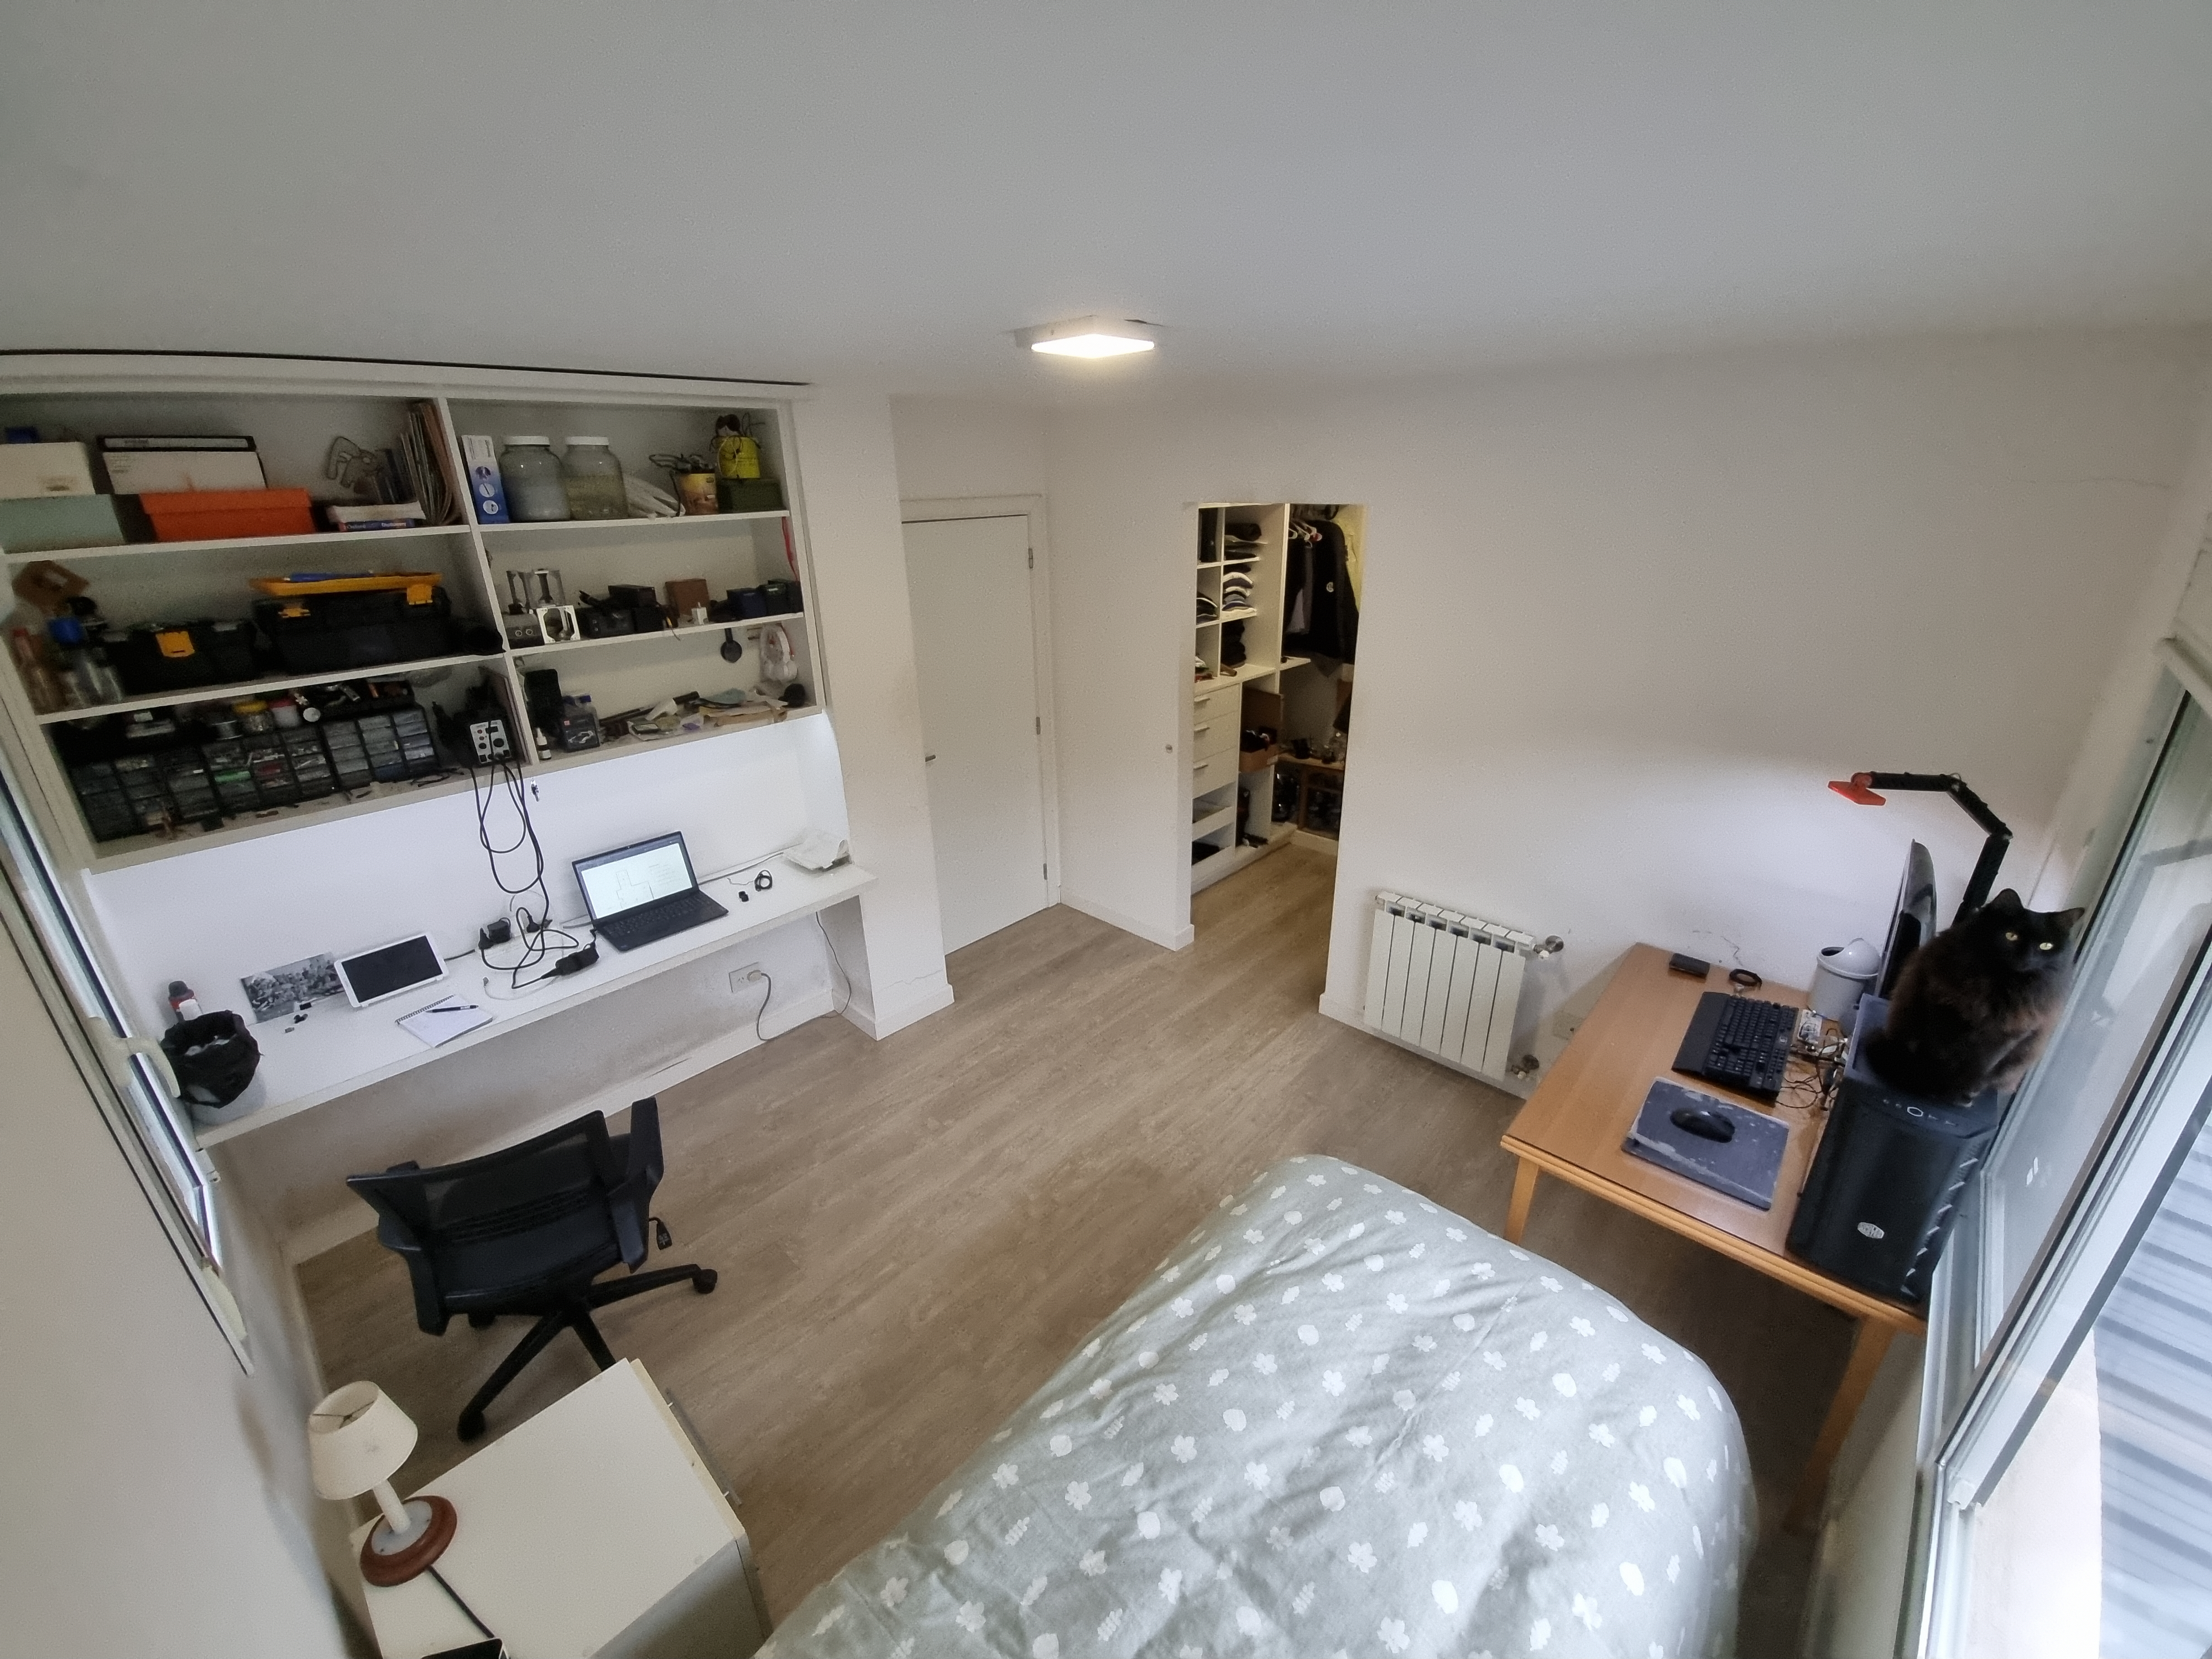
\includegraphics[width=\textwidth]{pictures/foto_oficina.jpg}
        \caption{Fotografía de la oficina técnica.}
        \label{fig.tp2:foto_oficina}
    \end{subfigure}
    \hfill
    \begin{subfigure}[t]{0.48\textwidth}
        \centering
        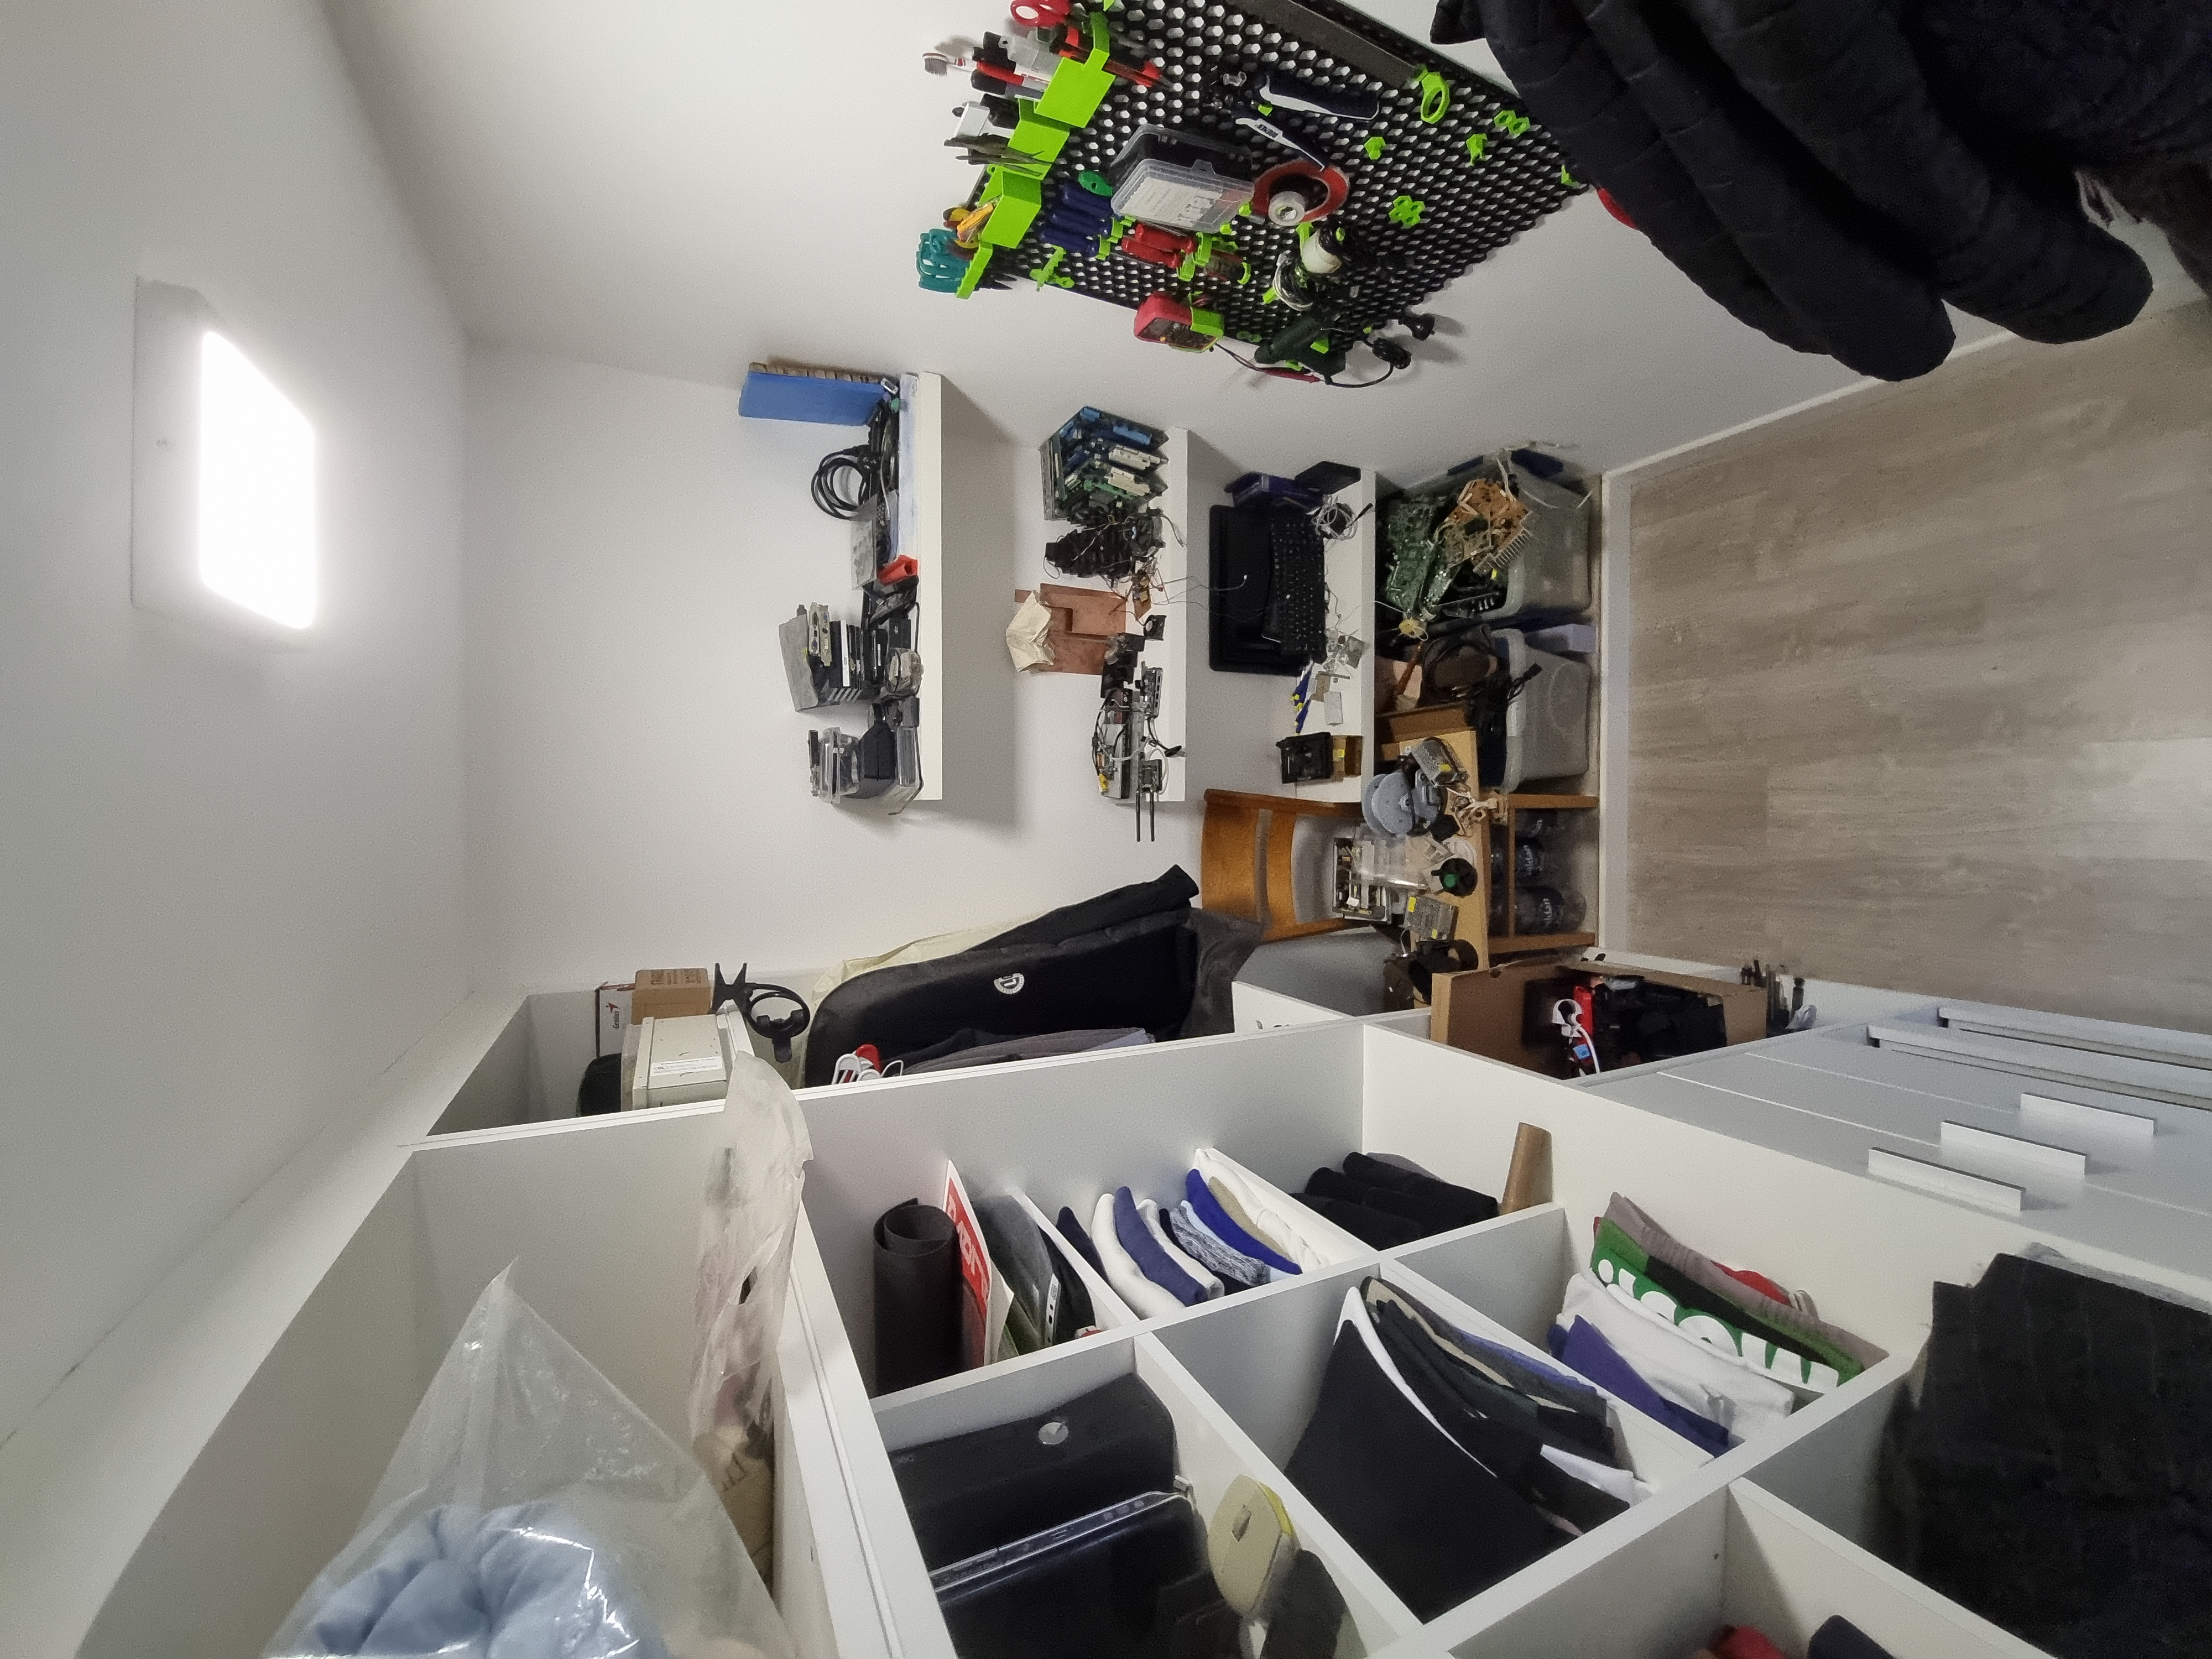
\includegraphics[width=\textwidth]{pictures/foto_deposito.jpg}
        \caption{Fotografía del depósito.}
        \label{fig.tp2:foto_deposito}
    \end{subfigure}
    \caption{Relevamiento fotográfico de los sectores de la habitación.}
    \label{fig.tp2:fotos_relevamiento}
\end{figure}

\chapter{Relevamiento de Mediciones}
\label{sec.tp2:mediciones}

En esta sección se presentan las planillas de registro de iluminancia de acuerdo con el formato y los requisitos
establecidos en el protocolo obligatorio de la Resolución SRT N° 84/2012, agregando las columnas normativas
necesarias.

\section{Planilla de Registro de Iluminancia (Protocolo Res. SRT 84/2012)}
\label{sec.tp2:registro_mediciones}

La Tabla~\ref{tab.tp2:tabla_mediciones_grilla} contiene el listado de puntos generales y localizados relevados. Para cada
punto se indica su designación, sus coordenadas de posición ($x, y$) referenciadas al croquis de la
Figura~\ref{fig.tp2:croquis_habitacion}, el puesto de trabajo o sector asociado, y los campos requeridos por la
Resolución SRT N° 84/2012 para que el muestreo tenga validez legal.

\begin{table}[!ht]
\centering
\caption{Planilla de mediciones conforme al Protocolo de la Resolución SRT N° 84/2012.}
\label{tab.tp2:tabla_mediciones_grilla}
\resizebox{\textwidth}{!}{
\begin{tabular}{|c|c|c|c|c|c|c|c|c|c|}
\hline
\textbf{Punto} & \textbf{Coordenadas} & \textbf{Sector / Puesto} & \textbf{Hora} & \textbf{Tipo Ilum.} & \textbf{Tipo Fuente} & \textbf{Ilum.} & \textbf{Valor Medido} & \textbf{Valor Exigido} & \textbf{¿Cumple?} \\
& \textbf{($x, y$) [$\m$]} & \textbf{de Trabajo} & & \textbf{(Nat/Art/Mix)} & \textbf{(LED/Desc/Inc)} & \textbf{(Gral/Local)} & \textbf{[$\lx$]} & \textbf{[$\lx$]} & \textbf{(S/N)} \\ \hline
\hline
$E_{1}$ & $(0{,}587; 0{,}547)$ & Oficina - Area de Tránsito & 11:15 & Mix & LED & Gral & $316$ & $300$ & S \\ \hline
$E_{2}$ & $(1{,}760; 0{,}547)$ & Oficina - Area de Tránsito & 11:16 & Mix & LED & Gral & $188$ & $300$ & N \\ \hline
$E_{3}$ & $(2{,}933; 0{,}547)$ & Oficina - Area de Tránsito & 11:17 & Mix & LED & Gral & $250$ & $300$ & N \\ \hline
$E_{4}$ & $(0{,}587; 1{,}640)$ & Oficina - Area de Tránsito & 11:18 & Mix & LED & Gral & $212$ & $300$ & N \\ \hline
$E_{5}$ & $(1{,}760; 1{,}640)$ & Oficina - Centro General  & 11:19 & Mix & LED & Gral & $351$ & $300$ & S \\ \hline
$E_{6}$ & $(2{,}933; 1{,}640)$ & Oficina - Area de Tránsito & 11:20 & Mix & LED & Gral & $850$ & $300$ & S \\ \hline
$E_{7}$ & $(0{,}587; 2{,}733)$ & Oficina - Area de Tránsito & 11:21 & Mix & LED & Gral & $1311$ & $300$ & S \\ \hline
$E_{8}$ & $(1{,}760; 2{,}733)$ & Oficina - Area de Tránsito & 11:22 & Mix & LED & Gral & $1851$ & $300$ & S \\ \hline
$E_{9}$ & $(2{,}933; 2{,}733)$ & Oficina - Area de Tránsito & 11:22 & Mix & LED & Gral & $601$ & $300$ & S \\ \hline
\hline
$E_{10}$ & $(0{,}732; 3{,}720)$ & Depósito - Paso / Estante   & 11:25 & Art & LED & Gral & $157$ & $100$ & S \\ \hline
$E_{11}$ & $(1{,}115; 3{,}720)$ & Depósito - Paso / Estante   & 11:25 & Art & LED & Gral & $163$ & $100$ & S \\ \hline
$E_{12}$ & $(1{,}498; 3{,}720)$ & Depósito - Paso / Estante   & 11:26 & Art & LED & Gral & $331$ & $100$ & S \\ \hline
$E_{13}$ & $(0{,}732; 4{,}360)$ & Depósito - Paso / Estante   & 11:26 & Art & LED & Gral & $200$ & $100$ & S \\ \hline
$E_{14}$ & $(1{,}115; 4{,}360)$ & Depósito - Centro General   & 11:27 & Art & LED & Gral & $229$ & $100$ & S \\ \hline
$E_{15}$ & $(1{,}498; 4{,}360)$ & Depósito - Paso / Estante   & 11:27 & Art & LED & Gral & $190$ & $100$ & S \\ \hline
$E_{16}$ & $(0{,}732; 5{,}000)$ & Depósito - Paso / Estante   & 11:28 & Art & LED & Gral & $200$ & $100$ & S \\ \hline
$E_{17}$ & $(1{,}115; 5{,}000)$ & Depósito - Paso / Estante   & 11:28 & Art & LED & Gral & $140$ & $100$ & S \\ \hline
$E_{18}$ & $(1{,}498; 5{,}000)$ & Depósito - Paso / Estante   & 11:29 & Art & LED & Gral & $170$ & $100$ & S \\ \hline
\hline
$E_{L1}$ & $(0{,}250; 0{,}310)$ & Escritorio Largo - Sur      & 11:23 & Mix & LED & Local & $335$ & $500$ & N \\ \hline
$E_{L2}$ & $(0{,}250; 0{,}940)$ & Escritorio Largo - Centro   & 11:23 & Mix & LED & Local & $355$ & $500$ & N \\ \hline
$E_{L3}$ & $(0{,}250; 1{,}570)$ & Escritorio Largo - Norte    & 11:24 & Mix & LED & Local & $347$ & $500$ & N \\ \hline
\hline
$E_{C1}$ & $(3{,}140; 2{,}680)$ & Escritorio Chico - Centro   & 11:24 & Mix & LED & Local & $710$ & $500$ & S \\ \hline
\end{tabular}
}
\end{table}

\section{Resumen de Cálculos y Parámetros del Protocolo}
\label{sec.tp2:resumen_resultados_calculados}

A partir de las mediciones registradas, se calcularon los valores promedio y las relaciones de uniformidad por sector:

\subsection{Sector Oficina (Iluminación General)}
\begin{itemize}
    \item Sumatoria de valores medidos:
    \begin{equation}
        \sum_{i=1}^{9} E_i = 5930 \lx
    \end{equation}
    \item Iluminancia media ($E_{media,of}$):
    \begin{equation}
        E_{media,of} = \frac{1}{9} \sum_{i=1}^{9} E_i = 658{,}89 \lx
    \end{equation}
    \item Iluminancia mínima registrada ($E_{min,of}$):
    \begin{equation}
        E_{min,of} = 188 \lx
    \end{equation}
    \item Relación de uniformidad exigida ($E_{media,of}/2$):
    \begin{equation}
        \frac{E_{media,of}}{2} = 329{,}44 \lx
    \end{equation}
\end{itemize}

\subsection{Sector Depósito (Iluminación General)}
\begin{itemize}
    \item Sumatoria de valores medidos:
    \begin{equation}
        \sum_{i=10}^{18} E_i = 1780 \lx
    \end{equation}
    \item Iluminancia media ($E_{media,dep}$):
    \begin{equation}
        E_{media,dep} = \frac{1}{9} \sum_{i=10}^{18} E_i = 197{,}78 \lx
    \end{equation}
    \item Iluminancia mínima registrada ($E_{min,dep}$):
    \begin{equation}
        E_{min,dep} = 140 \lx
    \end{equation}
    \item Relación de uniformidad exigida ($E_{media,dep}/2$):
    \begin{equation}
        \frac{E_{media,dep}}{2} = 98{,}89 \lx
    \end{equation}
\end{itemize}

\subsection{Iluminación Localizada en Puestos de Trabajo}
\begin{itemize}
    \item \textbf{Escritorio Largo (Tira LED):}
    \begin{equation}
        E_{media,L} = \frac{E_{L1} + E_{L2} + E_{L3}}{3} = 345{,}67 \lx
    \end{equation}
    \item \textbf{Escritorio Chico (Mesa):}
    \begin{equation}
        E_{C1} = 710 \lx
    \end{equation}
\end{itemize}

\chapter{Análisis de Resultados}
\label{sec.tp2:analisis}

En este capítulo se realiza la verificación comparativa de las mediciones registradas frente a los límites mínimos
exigidos por el Decreto N° 351/79 (Anexo IV) para garantizar la aptitud higiénica de las condiciones laborales.

\section{Límites Legales de Referencia}
\label{sec.tp2:limites_legales}

De acuerdo con la Tabla 2 del Anexo IV del Decreto N° 351/79, los valores mínimos de iluminancia exigidos ($E_{req}$) son:
\begin{itemize}
    \item \textbf{Oficina (Iluminación General):} $E_{req} = 300\lx$ (lectura y escritura general de oficina).
    \item \textbf{Depósito (Iluminación General):} $E_{req} = 100\lx$ (depósitos de mercadería o tránsito de personas).
    \item \textbf{Escritorio Largo (Iluminación Localizada):} $E_{req} = 500\lx$ (tareas de diseño técnico y dibujo de precisión).
    \item \textbf{Escritorio Chico (Iluminación Localizada):} $E_{req} = 500\lx$ (tareas de dibujo técnico o $300\lx$ para tareas administrativas generales).
\end{itemize}

\section{Planilla de Verificación Normativa}
\label{sec.tp2:verificacion_normativa}

En la Tabla~\ref{tab.tp2:verificacion_ley} se presenta la comparación de los valores medidos y calculados frente a las exigencias del Decreto N° 351/79, detallando su conformidad.

\begin{table}[!ht]
\centering
\caption{Comparación de mediciones contra las exigencias del Decreto N° 351/79.}
\label{tab.tp2:verificacion_ley}
\resizebox{0.95\textwidth}{!}{
\begin{tabular}{|l|l|c|c|c|}
\hline
\textbf{Sector} & \textbf{Criterio de Control} & \textbf{Valor Medido/Calculado} & \textbf{Límite Legal} & \textbf{Estado} \\ \hline
\hline
& Iluminancia Media ($E_{media,of}$) & $658{,}89\lx$ & $\ge 300\lx$ & \textbf{Cumple} \\ \cline{2-5}
\textbf{Oficina} & Iluminancia Mínima ($E_{min,of}$)   & $188\lx$ & $\ge 329{,}44\lx$ & \textbf{No Cumple} \\ \hline
\hline
& Iluminancia Media ($E_{media,dep}$) & $197{,}78\lx$ & $\ge 100\lx$ & \textbf{Cumple} \\ \cline{2-5}
\textbf{Depósito} & Iluminancia Mínima ($E_{min,dep}$)   & $140\lx$ & $\ge 98{,}89\lx$ & \textbf{Cumple} \\ \hline
\hline
\textbf{Escritorio Largo} & Iluminancia Localizada ($E_{media,L}$) & $345{,}67\lx$ & $\ge 500\lx$ & \textbf{No Cumple} \\ \hline
\hline
\textbf{Escritorio Chico} & Iluminancia Localizada ($E_{C1}$) & $710\lx$ & $\ge 500\lx$ & \textbf{Cumple} \\ \hline
\end{tabular}
}
\end{table}

\section{Interpretación y Diagnóstico}
\label{sec.tp2:interpretacion_diag}

A partir de los resultados expuestos en la Tabla~\ref{tab.tp2:verificacion_ley}, se desprende el siguiente diagnóstico técnico para cada uno de los sectores relevados:

\subsection{Sector Oficina}
\begin{itemize}
    \item \textbf{Iluminancia Media ($E_{media,of} = 658{,}89\lx$):} El nivel medio de iluminancia cumple holgadamente con el mínimo legal de $300\lx$. Esto se debe a la significativa contribución de luz natural que ingresa a través de los ventanales laterales durante la mañana tardía (rango de medición 11:15 a 11:22 Hs).
    \item \textbf{Criterio de Uniformidad ($E_{min,of} = 188\lx$ vs. $E_{media,of}/2 = 329{,}44\lx$):} Este parámetro \textbf{no cumple} con las exigencias del Decreto N° 351/79. Se observa una marcada dispersión entre los puntos cercanos a las ventanas ($E_7 = 1311\lx$ y $E_8 = 1851\lx$) y los puntos más alejados o en zonas sombreadas ($E_2 = 188\lx$ y $E_4 = 212\lx$), los cuales dependen casi de forma exclusiva del único plafón LED general de $18\W$. Esta falta de uniformidad representa un riesgo ergonómico para el personal debido a la fatiga visual por acomodación pupilar frecuente y al deslumbramiento por contraste.
\end{itemize}

\subsection{Sector Depósito}
\begin{itemize}
    \item El depósito es un local cerrado sin aberturas al exterior, por lo que su iluminación es 100\% artificial. El promedio general es de $197{,}78\lx$, superando el requisito legal de $100\lx$. 
    \item El criterio de uniformidad se satisface plenamente ($E_{min,dep} = 140\lx \ge 98{,}89\lx$). El plafón LED central de $18\W$ proporciona una distribución lumínica muy homogénea y adecuada para las tareas de almacenamiento y tránsito seguro de mercaderías.
\end{itemize}

\subsection{Puestos de Trabajo (Iluminación Localizada)}
\begin{itemize}
    \item \textbf{Escritorio Largo (Tira LED):} La iluminancia media sobre el plano de trabajo es de $345{,}67\lx$, valor que se encuentra \textbf{por debajo} del límite reglamentario de $500\lx$ para tareas que exijan precisión visual. A pesar del montaje directo a $62\cm$, la potencia luminosa y densidad de la tira LED actual son deficientes frente a las exigencias visuales del puesto.
    \item \textbf{Escritorio Chico (Mesa):} El puesto registra $710\lx$ en su centro de trabajo, superando satisfactoriamente el límite de $500\lx$. La lámpara regulable resulta muy efectiva gracias a su elevado flujo luminoso ($700\lm$) y a la posibilidad de orientar y aproximar la fuente puntual según los requerimientos del operador.
\end{itemize}

\chapter{Conclusiones y Recomendaciones}
\label{sec.tp2:conclusiones}

Este capítulo compila la evaluación conclusiva de la instalación de iluminación relevada en base a las mediciones
registradas y al análisis comparativo con el marco legal.

\section{Conclusión del Relevamiento}
\label{sec.tp2:conclusion_evaluacion}

Luego de procesar y evaluar las mediciones realizadas en el local, se determinan las siguientes conclusiones técnicas:
\begin{itemize}
    \item \textbf{Sector Oficina:} La iluminancia media general es satisfactoria ($658{,}89\lx \ge 300\lx$), pero \textbf{no cumple con el criterio de uniformidad legal} debido al fuerte contraste provocado por la radiación solar directa que ingresa por las ventanas. Las zonas más alejadas de las aberturas dependen únicamente del plafón central de $18\W$ y registran niveles insuficientes ($188\lx$), por lo que existe riesgo de fatiga visual y deslumbramiento.
    \item \textbf{Sector Depósito:} El sector \textbf{cumple plenamente} con el marco legal (Dec. N° 351/79), tanto en nivel medio ($197{,}78\lx \ge 100\lx$) como en uniformidad ($140\lx \ge 98{,}89\lx$). La iluminación artificial general es adecuada y homogénea.
    \item \textbf{Escritorio Largo (Puesto Localizado):} El puesto \textbf{no cumple} con las exigencias legales para dibujo y diseño técnico ($345{,}67\lx < 500\lx$). La tira LED de $5050$ actual es insuficiente a la altura de montaje de $62\cm$.
    \item \textbf{Escritorio Chico (Puesto Localizado):} El puesto \textbf{cumple satisfactoriamente} con el nivel exigido de $500\lx$, alcanzando una iluminancia de $710\lx$ gracias al correcto funcionamiento y direccionamiento de la luminaria de mesa regulable de $700\lm$.
\end{itemize}

\section{Medidas de Recomendación y Mejora}
\label{sec.tp2:recomendaciones}

Con el fin de subsanar los desvíos detectados y optimizar las condiciones ergonómicas y de seguridad del local, se recomiendan las siguientes acciones correctivas y preventivas:

\begin{enumerate}
    \item \textbf{Readecuación de la Iluminación General de la Oficina:} Se aconseja instalar un segundo plafón LED de $18\W$ en el cielorraso de la oficina, disponiéndolos simétricamente. Esto reforzará los niveles de iluminancia artificial en las zonas alejadas de la ventana (puntos $E_2, E_3, E_4$), elevándolos sobre los $300\lx$ y garantizando una óptima relación de uniformidad ($E_{min} \ge E_{media}/2$).
    \item \textbf{Control de la Luz Natural Directa:} Implementar cortinas translúcidas, persianas regulables o vinilos difusores en las ventanas (en especial la ventana de la derecha). Esto atenuará los picos excesivos de radiación solar directa ($1851\lx$) que causan deslumbramiento y elevados contrastes térmicos y lumínicos.
    \item \textbf{Reemplazo de la Tira LED en el Escritorio Largo:} Sustituir la tira LED $5050$ actual por una tira LED de mayor flujo luminoso y densidad (por ejemplo, una tira de tecnología SMD 2835 o de doble hilera con una densidad de $120\text{ leds}/\m$ o superior). Esto aumentará la iluminancia sobre el plano de trabajo por encima de los $500\lx$ requeridos para actividades visuales de precisión.
    \item \textbf{Programa de Limpieza Periódica:} Establecer un cronograma semestral de limpieza de difusores y lámparas para evitar la pérdida de rendimiento por sedimentación de polvo (depreciación del flujo luminoso).
    \item \textbf{Monitoreo Anual Obligatorio:} Programar nuevas mediciones preventivas con frecuencia anual, de acuerdo con las directrices de la Resolución SRT N° 84/2012, para verificar la constancia de las condiciones lumínicas del ambiente de trabajo.
\end{enumerate}


\nocite{*}
\printbibliography[heading=bibnumbered, title={Fuentes}]

\end{document}
